\newpage
\section{Altre tecniche}
\subsection{Dependency injection}
\begin{itemize}
	\item \textbf{Scopo}: questa tecnica permette di applicare il principio di \termine{Inversion of Control}, e consiste nel fornire agli oggetti che presentano dipendenze verso altri oggetti tali dipendenze senza lasciare che siano i primi a crearle, ma facendo sì che sia un terzo oggetto a fornirle.
	\item \textbf{Motivazione}: lasciare al componente il compito di risolvere le proprie dipendenze, creando
gli oggetti necessari al suo funzionamento, aumenta l'accoppiamento tra le componenti e
rende più difficoltoso progettare i test di unità. Tramite l'utilizzo di questo pattern invece è possibile esprimere
le dipendenze in modo dichiarativo e utilizzare un oggetto contenitore per risolverle
dinamicamente a tempo di esecuzione. In questo modo è possibile scegliere anche quale componente
iniettare in base allo stato del programma.
	\item \textbf{Applicabilità}: questa tecnica può essere applicata all'interno di tutte quelle applicazioni che presentano un alto grado di accoppiamento tra le varie classi, per rilassare queste dipendenze. E' bene notare che, essendo necessaria una libreria di terze parti per applicare questa tecnica, essa non è applicabile a tutti i linguaggi di programmazione. Per il progetto, il \termine{gruppo} ha deciso di utilizzare la libreria \texttt{dependency-injection-es6};
	\item \textbf{Struttura}: i componenti coinvolti nella \termine{Dependency Injection} sono: 
	\begin{itemize}
		\item Un \textbf{client} che viene creato e riceve le dipendenze.
		\item Un \textbf{contenitore} che si occupa di creare il client e di iniettarvi le dipendenze.
		\item Un \textbf{servizio} che deve essere iniettato al client.
	\end{itemize}
	Nello specifico di \texttt{dependency-injection-es6}, \texttt{container} funziona da contenitore che si occupa di risolvere le dipendenze. I client sono rappresentati dalle funzioni che costruiscono i componenti dell'applicazione, tipicamente Presenter, \termine{Use case} o \termine{Source}. Il servizio è una classe definita dall'utente che esegue le azioni desiderate. \\
	\begin{figure}[ht]
	\centering
	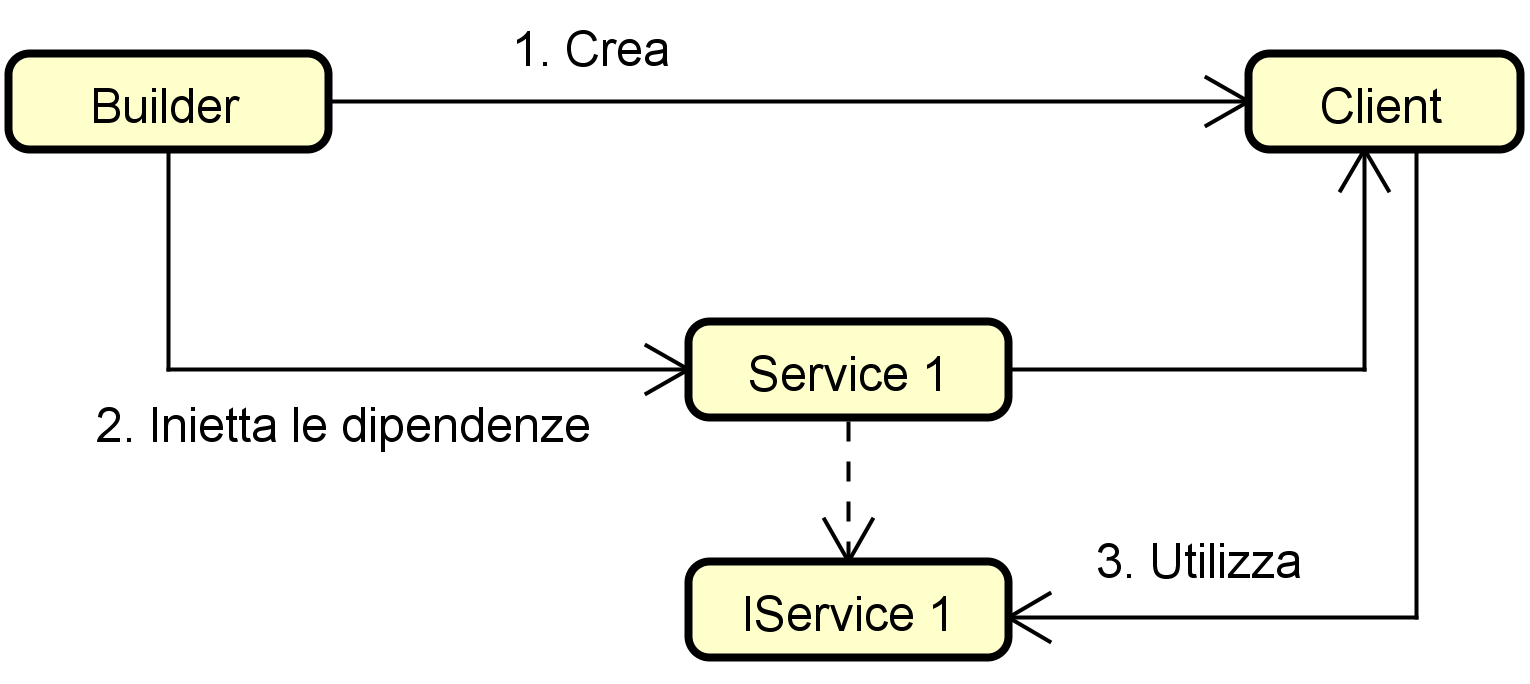
\includegraphics[scale=0.25]{Sezioni/DesignPatterns/DependencyInjection.png}
	\caption{Struttura logica della tecnica di Dependency Injection}
	\end{figure}
	L'injection delle dipendenze può essere fatta in due modi:
	\begin{itemize}
	 	\item \textbf{Constructor Injection}: le dipendenze vengono dichiarate come parametri del costruttore
che il container andrà a valorizzare quando crea l’oggetto. In questo modo l’oggetto costruito è subito utilizzabile e non è mai in uno stato inconsistente. Tuttavia
si rende necessario avere dei costruttori con un elevato numero di parametri, che
potrebbero rendere i costruttori difficili da comprendere.
 	 	\item \textbf{Field injection}: le dipendenze vengono dichiarate come semplici campi dati all'interno della classe contenitore. Questa situazione permette di poter mantenere un costruttore senza parametri, ma nasconde le dipendenze effettive che vi sono tra la classe che la sfrutta e i vari servizi iniettati.
	\end{itemize}
	
	\item \textbf{Utilizzo}: questa tecnica viene utilizzata all'interno delle classi che rappresentano l'implementazione delle interfacce delle viste secondo il metodo della \textbf{Field Injection} per ottenere le istanze del \termine{Presenter} al quale sono legate. Inoltre è utilizzata a cascata la tecnica di \textbf{Constructor Injection} per costruire le varie classi \termine{Presenter} e tutte le classi che si incontrano nel grafo delle dipendenze.
	\item \textbf{Svantaggi}: eventuali errori legati alla risoluzione delle dipendenze o alla loro
implementazione vengono rilevati solamente durante l'esecuzione.
\end{itemize}